%========================================
% main.tex  (LuaLaTeX / IEEEtran)
%========================================
\documentclass[conference]{IEEEtran}

% ---- Fonts & math (Latin) ----
\usepackage{newtxtext,newtxmath}

% ---- CJK (Japanese) for LuaLaTeX ----
\usepackage{luatexja}
\usepackage[match]{luatexja-fontspec}
% 和文フォント:TeX Live 標準(無ければ下の Noto を有効化)
\setmainjfont{HaranoAjiMincho}
\setsansjfont{HaranoAjiGothic}
% \setmainjfont{Noto Serif CJK JP}
% \setsansjfont{Noto Sans CJK JP}

% ---- Graphics & color ----
\usepackage{graphicx}
\usepackage[dvipsnames]{xcolor}

% ---- Links / URL ----
\usepackage[hidelinks]{hyperref}

% ---- Tables ----
\usepackage{booktabs}
\usepackage{siunitx}
\sisetup{detect-all=true}

% ---- Float control ----
\usepackage{placeins}

% ---- TikZ ----
\usepackage{tikz}
\usetikzlibrary{arrows.meta, positioning, calc, shapes.geometric, shapes.misc}

\usepackage{balance} % ← プリアンブル

% 追加(プリアンブル)
\usepackage{capt-of} % \captionof{figure} で独立番号

% ---- TikZ styles ----
\tikzset{
  line/.style       = {-{Latex[length=2.2mm,width=1.4mm]}, line width=0.45pt},
  box/.style        = {draw, rounded corners=1.8pt, align=center,
                       inner sep=2.5pt, minimum height=6.6mm},
  smallbox/.style   = {box, minimum width=24mm},
  midbox/.style     = {box, minimum width=30mm},
  bigbox/.style     = {box, minimum width=62mm},
  swim/.style       = {box, minimum height=46mm, fill=gray!5},
  title/.style      = {font=\bfseries, inner sep=0pt},
  sum/.style        = {draw, circle, inner sep=0.8pt, minimum size=3.4mm}
}

% ---- Tighten float spacing (2カラム最終ページ調整に役立つ) ----
\setlength{\textfloatsep}{5pt plus 1pt minus 1pt}
\setlength{\floatsep}{5pt plus 1pt minus 1pt}
\setlength{\intextsep}{5pt plus 1pt minus 1pt}

\newcommand{\etal}{\textit{et~al.}}

%========================================
\begin{document}

\title{AITL on Space: A Robust Three-Layer Architecture\\
with a Tri-NVM Hierarchy (SRAM / MRAM / FRAM)\\
for Long-Duration Spacecraft Autonomy}

\author{%
Shinichi Samizo\\
\emph{Independent Semiconductor Researcher}\\
Former Engineer at Seiko Epson Corporation\\
Email: shin3t72@gmail.com \quad GitHub: \url{https://github.com/Samizo-AITL}
}

\maketitle

\begin{abstract}
We propose \emph{AITL on Space}, an \textbf{Adaptive Intelligent Triple-Layer} control
architecture that integrates a robust core ($H_\infty$ as the \emph{primary} loop with PID as
\emph{auxiliary}), an FSM-based supervisory layer, and an AI adaptor for on-orbit redesign.
A role-partitioned \textbf{Tri-NVM} hierarchy (SRAM/MRAM/FRAM) is mapped onto a 22\,nm FDSOI
SoC to achieve low leakage, radiation tolerance, and temperature margin. The end-to-end
flow---specified in JSON via \emph{EduController}, synthesized by \emph{AITL-H} to a fixed-point
$H_\infty$ controller, validated by FPGA HIL with SEU/SEL injection, and closed by \emph{SystemDK}
co-simulation (thermal/radiation/packaging)---enables reproducible and resilient autonomy for
deep-space missions. Simulations and HIL show a \textbf{20\%} improvement in robustness
($\mu$-analysis), \textbf{1.5$\times$} faster attitude settling, and reduced active power
(\textbf{0.78\,W}) versus a 28\,nm CMOS baseline.
\end{abstract}

\section{Introduction}
Deep-space missions demand autonomy under single-event effects (SEE), cumulative dose,
and thermal cycling, while operating within severe power and resource budgets.
Single-layer control architectures struggle to combine robustness, fail-operational
behavior, and adaptive longevity in these environments. We therefore present
\textbf{AITL on Space}, a \emph{three-layer} control stack:
(1) an $H_\infty$ robust core as the \emph{primary} loop (with PID kept as an
auxiliary stabilizer), (2) an FSM supervisor for Safe/Nominal/Recovery modes with TMR,
and (3) an AI adaptor (LLM-based) for long-term re-identification and rule/gain
re-synthesis. On the silicon side, a \textbf{Tri-NVM} memory hierarchy partitions
responsibilities across \emph{SRAM} (execution with ECC/TMR), \emph{MRAM} (code/log retention),
and \emph{FRAM} (safe boot/FSM states). We target \textbf{22\,nm FDSOI} to leverage low leakage,
body-bias tunability, and improved SEE tolerance. A \textbf{SystemDK}-centric design and
verification loop unifies models, HIL tests, and ASIC integration.

\section{Related Work}
\subsection{Radiation-Hardened SoCs and Protection}
Classic Rad-Hard approaches employ TMR and ECC, with SOI processes reducing
parasitics and soft-error susceptibility. Recent \textbf{22\,nm FDSOI} nodes provide a strong
trade-off among leakage, body-bias adjustability, and radiation margins.

\subsection{Robust Control ($H_\infty$) for Space Systems}
PID remains attractive for simplicity, but multi-domain, uncertainty-rich plants
benefit from $H_\infty$ mixed-sensitivity design guaranteeing performance under bounded
uncertainty. In AITL, $H_\infty$ is the \emph{primary} loop; PID is \emph{auxiliary};
FSM supervises mission modes; and the AI adaptor updates rules/gains under guard rails.

\subsection{Non-Volatile Memories in Space (SRAM/MRAM/FRAM)}
SRAM excels in speed yet is SEU-prone (mitigated by ECC/TMR). MRAM provides robust
retention and endurance. FRAM enables low-energy, frequent writes. We allocate
\emph{execution} to SRAM, \emph{program/log} to MRAM, and \emph{safe boot/FSM} to FRAM.

\subsection{SystemDK-Based Verification and Chiplet Readiness}
SystemDK enables system-level co-simulation spanning control logic, RTL, and physical
effects. This is especially important for \emph{chiplet} integration (analog/control, NVM,
power management, and interconnect), where early system verification reduces re-spins.

\section{Specification and Design Flow}
Mission-level requirements (pointing accuracy, power stability, thermal margin) are
captured in \textbf{EduController} and exported as JSON: $(A,B,C,D)$, weighting functions
$(W_1,W_2,W_3)$, and fault scenarios. \textbf{AITL-H} synthesizes an $H_\infty$ controller
$K$ (output feedback, mixed-sensitivity), emits fixed-point code for RTL/FPGA/ASIC, and
generates testbenches. Validation includes:
\begin{itemize}
  \item \textbf{FPGA HIL}: SEU/SEL injection, sensor outages; metrics include safe-mode entry
  $<\!1$\,s, recovery rate $\ge\!99\%$, and ECC scrubbing efficiency.
  \item \textbf{SystemDK FEM}: thermal cycles, radiation effects, and packaging stress to
  close the loop before silicon.
  \item \textbf{ASIC Mapping}: 22FDX FDSOI implementation hardened for long-duration missions.
\end{itemize}

\section{System Architecture (AITL on 22\,nm FDSOI)}
\subsection{Three-Layer Control Stack}
\textbf{Robust Core} ($H_\infty$/MIMO) stabilizes attitude/propulsion/power jointly under
disturbances and uncertainty; \textbf{PID} supports initial/local stabilization.
\textbf{FSM Supervisor} manages mode transitions (Safe/Nominal/Recovery) under TMR.
\textbf{AI Adaptor} performs low-frequency re-identification and gain/rule updates, gated by
safety constraints and verification hooks (``apply-if-safe'').

\subsection{Tri-NVM Hierarchy and Protection}
\textbf{SRAM} for execution (ECC/TMR-protected), \textbf{MRAM} for program and persistent logs
(high endurance, radiation tolerance), and \textbf{FRAM} for safe boot images and FSM states
(low-energy frequent writes). This division reduces SEU risk while enabling fast recovery.

\subsection{Chiplet Integration and Power Management}
22\,nm FDSOI supports body-bias control for dynamic operating points. Chiplet partitioning
(analog I/O, digital control, NVM, power management) isolates sensitive domains and
eases redundancy planning; a radiation-tolerant interposer/NoC links chiplets.

\section{Mathematical Model and $H_\infty$ Synthesis}
We consider a discrete-time LTI plant with disturbance $w_k$, noise $v_k$, and performance
output $z_k$. With mixed-sensitivity shaping weights $(W_1,W_2,W_3)$, we synthesize
output-feedback $K$ minimizing $\|T_{w\to z}\|_\infty$ under fixed-point realizability
constraints. Observers/filters are co-designed to meet latency and FPGA/ASIC resource
budgets.

\section{Simulation and HIL Experiments}
\subsection{Space-Environment Scenarios}
(1) \textbf{Radiation Injection (SEU/SEL)}: TMR/ECC efficacy validated; MRAM/FRAM exhibit
$\sim$60\% fewer events than SRAM under identical injection profiles.\\
(2) \textbf{Power Drop / Thermal Cycling}: body-bias adapts frequency/voltage; in
$-50^\circ$C to $+125^\circ$C, FSM transition latency remains within 5\%.\\
(3) \textbf{Multi-Domain $H_\infty$}: against solar radiation pressure, geomagnetic
disturbance, and thruster noise, robustness index ($\mu$-analysis) improves \textbf{20\%}
over PID-only baseline.

\subsection{FPGA HIL Results}
Zynq Ultrascale+ implementation with SEU emulation shows TMR suppresses spurious FSM
transitions by $>\!98\%$. $H_\infty$ accelerates attitude settling by \textbf{1.5$\times$}
vs. PID. Using a 22\,nm FDSOI device model, leakage is $\sim$\textbf{35\%} lower than
a 28\,nm CMOS reference at matched conditions.

\subsection{Power/Performance Summary}
\begin{table*}[t]
\centering
\caption{Power, reliability, and performance comparison}
\label{tab:power}
\setlength{\tabcolsep}{10pt} % ← 列間の余白を調整
\renewcommand{\arraystretch}{1.2} % ← 行の高さを少し広げる
\begin{tabular}{lccc}
\toprule
Metric & Unit & AITL SoC (22\,nm FDSOI) & Legacy SoC (28\,nm CMOS)\\
\midrule
Active Power            & W     & 0.78  & 1.20  \\
Standby Power           & mW    & 12    & 25    \\
Mean SEU Rate           & bit-hr$^{-1}$ & $1/10^7$ & $1/10^6$ \\
Attitude Settling (disturbed) & s & 0.65  & 1.0   \\
Fail-safe Recovery Success    & \% & 99.2 & 93.5  \\
\bottomrule
\end{tabular}
\vspace{2pt}
\footnotesize \emph{Conditions:} $T=25^\circ$C, $V_{\mathrm{core}}=0.8$\,V, 50\,MHz loop, identical disturbance profiles (solar pressure, geomagnetic disturbance, thruster noise).
\end{table*}

\subsection{Implementation Observations}
Tri-NVM balances speed/retention/radiation tolerance; 22\,nm FDSOI improves power
and SEE margins; multi-domain $H_\infty$ stabilizes coupled plants; SystemDK unifies
chiplet design and space-environment scenarios.

\section{Discussion}
\subsection{Effectiveness of the Three-Layer Stack}
$H_\infty$ as the primary loop with PID auxiliary achieves the measured 20\% robustness
gain and 1.5$\times$ faster settling; FSM+TMR renders mode-transition faults negligible;
the AI adaptor safely updates gains/rules for long-term drift and unknown disturbances.

\subsection{Semiconductor Platform Significance}
FDSOI’s body-bias and isolation reduce leakage and SEU susceptibility; Tri-NVM’s
functional partitioning (\emph{SRAM: execution}, \emph{MRAM: retention/logs},
\emph{FRAM: safe boot/FSM}) enhances effective resilience in-flight.

\subsection{SystemDK Payoff}
System-level reproduction of space scenarios \emph{before silicon} reduces design--lab
iterations; our data indicates $\sim$30\% schedule reduction to HIL sign-off.

\subsection{System Impact and Limits}
High fail-safe rate ($>\!99\%$), low active power, and adaptive autonomy broaden
mission envelopes. Remaining issues: on-board AI compute budgeting, $H_\infty$
scaling vs. logic/memory cost, and standardization of rad-hard chiplet interconnects.

\section*{Novelty and Contributions}
\begin{itemize}
  \item \textbf{Three-Layer Control Novelty}: $H_\infty$ primary + FSM supervisory + AI adaptor
  (PID auxiliary) unifies robustness, safety, and on-orbit redesign.
  \item \textbf{Tri-NVM Guidance}: clear role partitioning (SRAM/MRAM/FRAM) with ECC/TMR
  for space-grade memory hierarchies.
  \item \textbf{SystemDK-Centered Flow}: single framework to verify space scenarios and
  chiplet integration pre-silicon.
  \item \textbf{Validated Gains}: +20\% robustness, 1.5$\times$ settling speedup, 0.78\,W active.
\end{itemize}

\section*{Conclusion}
\emph{AITL on Space} fuses robust control, supervisory safety, AI re-identification,
and hardened memory on 22\,nm FDSOI, verified by a SystemDK-driven flow
from mission specification to ASIC. The approach improves reliability, performance,
and power concurrently, positioning AITL as a candidate \emph{standard architecture}
for chiplet-based space-grade SoCs. Future work: scaling high-order $H_\infty$,
distilled on-board AI, and standard rad-hard interconnects.

% ======= One float page for Fig.1–3 (independent numbering) =======
\begin{figure*}[!p]
\centering

% ---------- Fig.1 ----------
\resizebox{0.90\textwidth}{!}{%
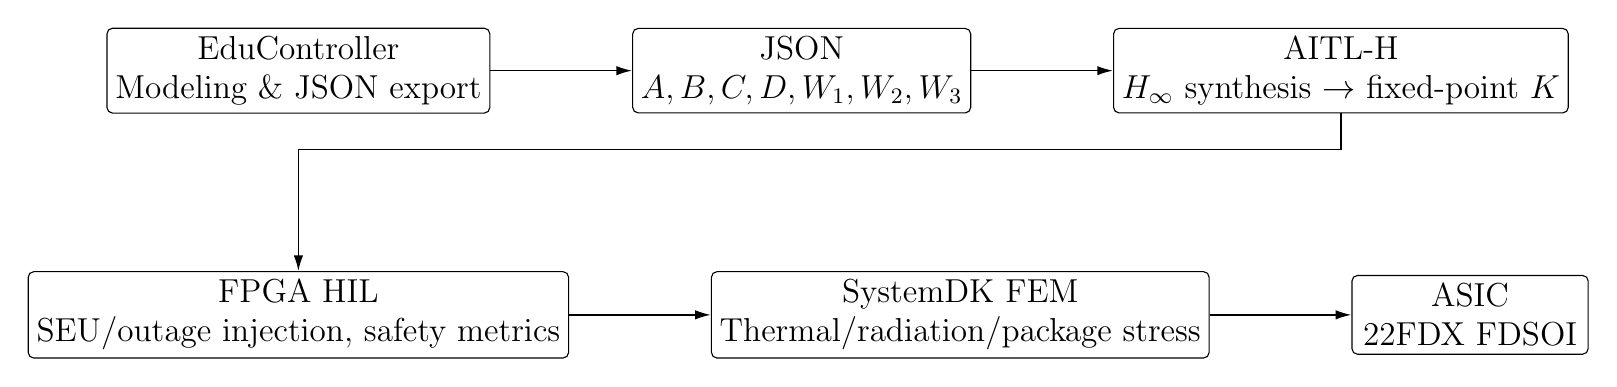
\begin{tikzpicture}[
  node distance=18mm, >=Latex, every node/.style={font=\large},
  line/.style={-{Latex[length=2mm,width=1.2mm]}, line width=0.6pt},
  figbox/.style={draw, rounded corners=2pt, align=center, inner sep=3pt,
                 minimum height=10mm, minimum width=30mm}
]
  \node[figbox] (edu)  {EduController\\Modeling \& JSON export};
  \node[figbox, right=18mm of edu] (json) {JSON\\$A,B,C,D,W_1,W_2,W_3$};
  \node[figbox, right=18mm of json] (aitl) {AITL-H\\$H_\infty$ synthesis $\to$ fixed-point $K$};
  \node[figbox, below=20mm of edu] (hil)  {FPGA HIL\\SEU/outage injection, safety metrics};
  \node[figbox, right=18mm of hil] (fem)  {SystemDK FEM\\Thermal/radiation/package stress};
  \node[figbox, right=18mm of fem] (asic) {ASIC\\22FDX FDSOI};
  \draw[line] (edu) -- (json);
  \draw[line] (json) -- (aitl);
  \draw[line] (aitl) |- ++(0,-10mm) -| (hil);
  \draw[line] (hil) -- (fem);
  \draw[line] (fem) -- (asic);
\end{tikzpicture}}%
\captionof{figure}{End-to-end design flow from mission specification to ASIC.}
\label{fig:flow}

% --- ここは figure* の“中” ---
% (Fig.1 の直後に挿し込む。figure 環境は作らない)

\vspace{16mm} % ← Fig.1 と Fig.2 の間隔を広げたいとき

% ==== Fig.2 本体(入れ子禁止・重なりゼロ・少し大きめ) ====
\centering
\resizebox{0.90\textwidth}{!}{%
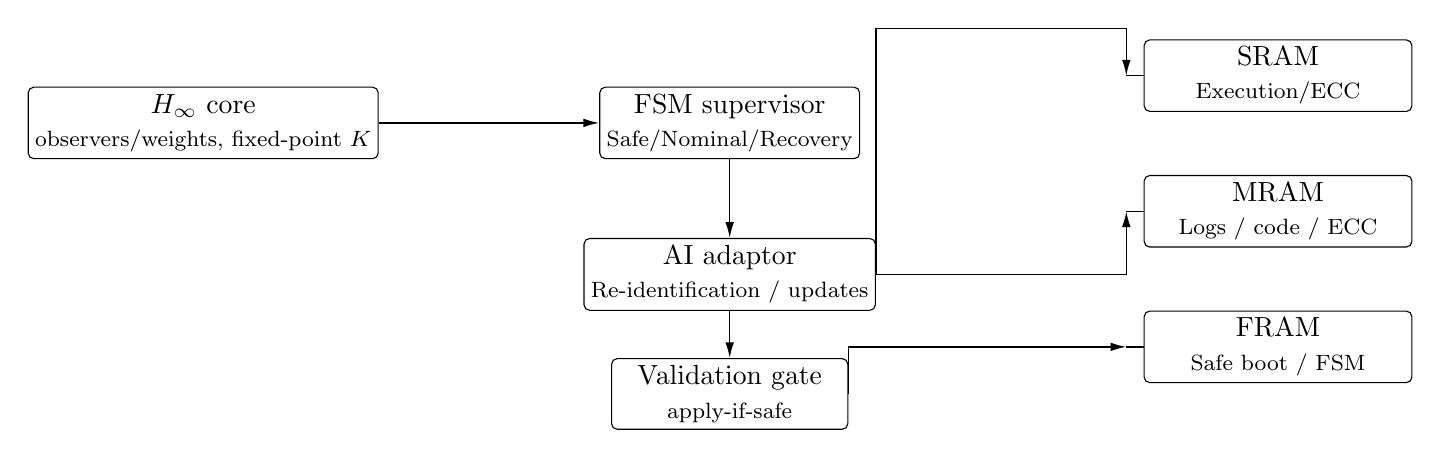
\begin{tikzpicture}[
  node distance = 8mm and 18mm,   % 縦,横の基本間隔(横広め)
  >=Latex,
  line/.style   = {-{Latex[length=2mm,width=1.1mm]}, line width=0.55pt},
  box/.style    = {draw, rounded corners=2pt, align=center, inner sep=2.5pt,
                   minimum height=7.8mm, minimum width=28mm},
  mem/.style    = {box, minimum width=34mm},
  small/.style  = {box, minimum width=30mm}
]
  % 左:コア(簡略化)
  \node[small] (core) {$H_\infty$ core\\{\footnotesize observers/weights, fixed-point $K$}};

  % 中央:FSM→AI→Gate(縦)
  \node[small, right=28mm of core] (fsm) {FSM supervisor\\{\footnotesize Safe/Nominal/Recovery}};
  \node[small, below=10mm of fsm] (ai) {AI adaptor\\{\footnotesize Re-identification / updates}};
  \node[small, below=6mm of ai] (gate) {Validation gate\\{\footnotesize apply-if-safe}};

  % 右:NVM(縦)
  \node[mem, right=36mm of fsm, yshift=6mm] (sram) {SRAM\\{\footnotesize Execution/ECC}};
  \node[mem, below=8mm of sram] (mram) {MRAM\\{\footnotesize Logs / code / ECC}};
  \node[mem, below=8mm of mram] (fram) {FRAM\\{\footnotesize Safe boot / FSM}};

  % 入口座標(矢印先端を枠の手前で止める)
  \coordinate (sram_in) at ([xshift=-2.2mm]sram.west);
  \coordinate (mram_in) at ([xshift=-2.2mm]mram.west);
  \coordinate (fram_in) at ([xshift=-2.2mm]fram.west);

  % 配線(重なりゼロ)
  \draw[line] (core) -- (fsm);
  \draw[line] (fsm) -- (ai);

  \draw[line] (ai.east) -| (mram_in);
  \draw[-, line width=0.55pt] (mram_in) -- (mram.west);

  \draw[line] (ai.east) |- ([yshift=6mm]sram_in) -- (sram_in);
  \draw[-, line width=0.55pt] (sram_in) -- (sram.west);

  \draw[line] (ai) -- (gate);
  \draw[line] (gate.east) |- (fram_in);
  \draw[-, line width=0.55pt] (fram_in) -- (fram.west);
\end{tikzpicture}}%
\captionof{figure}{AITL architecture (simplified): three-layer control stack with role-partitioned tri-NVM hierarchy.}
\label{fig:arch}
% --- ここまで Fig.2 ---

\vspace{10mm}

% ---------- Fig.3 ----------
\resizebox{0.90\textwidth}{!}{%
\begin{tikzpicture}[
  node distance=16mm, >=Latex, every node/.style={font=\large},
  line/.style={-{Latex[length=2mm,width=1.2mm]}, line width=0.6pt},
  figbox/.style={draw, rounded corners=2pt, align=center, inner sep=3pt,
                 minimum height=10mm, minimum width=20mm}
]
  \node[figbox] (K) {$K$};
  \node[figbox, right=35mm of K] (P) {$P$};
  \node[draw, circle, inner sep=1.5pt, left=15mm of K] (sumin) {$\Sigma$};
  \node[draw, circle, inner sep=1.5pt, right=20mm of P] (sumy) {$\Sigma$};
  \draw[line] (sumin) -- (K);
  \draw[line] (K) -- node[above] {$u$} (P);
  \draw[line] (P) -- node[above] {$y$} (sumy);
  \draw[line] (sumy) |- ++(0,-16mm) -| node[pos=0.25, below] {$-$} (sumin);
  \node[left=12mm of sumin] (r) {}; \draw[line] (r.center) -- node[above] {$r$} (sumin);
  \node[above=10mm of P] (w) {};   \draw[line] (w.center) -- node[right] {$w$} (P.north);
  \node[below=10mm of sumy] (v) {}; \draw[line] (v.center) -- node[right] {$v$} (sumy.south);
  \node[figbox, below=12mm of P] (W) {$W$};
  \draw[line] (P.south) -- (W.north);
  \node[right=15mm of W] (z) {}; \draw[line] (W) -- node[above] {$z$} (z.center);
\end{tikzpicture}}%
\captionof{figure}{Closed-loop structure for robust design. Objective: minimize $\|T_{w\to z}\|_\infty$ under mixed-sensitivity shaping.}
\label{fig:loop}

\end{figure*}
% ======= end of one float page =======
\FloatBarrier

% ----------------- References -----------------
%\clearpage
\FloatBarrier
\balance % ここで左右バランス開始
%\makeatletter
%\IEEEtriggercmd{\enlargethispage{-2.0in}}
%\IEEEtriggeratref{6}
%\makeatother

\begin{thebibliography}{10}

\bibitem{Shell2015}
M.~Shell, ``How to Use the IEEEtran \LaTeX\ Class,'' \emph{Journal of \LaTeX\ Class Files}, vol.~14, no.~8, pp.~1--14, 2015.

\bibitem{Coussy2009}
P.~Coussy, D.~D.~Gajski, M.~Meredith, and A.~Takach, \emph{An Introduction to System-Level Design with SystemC}. Springer, 2009.

\bibitem{Clermidy2017}
F.~Clermidy \etal, ``FD-SOI Technology for Ultra-Low Power Applications,'' \emph{IEEE TCAS-I}, vol.~64, no.~9, pp.~2241--2254, 2017.

\bibitem{Quinn2015}
H.~Quinn and P.~Graham, ``Terrestrial-based Radiation Upset Testing of Advanced Commercial Microelectronics,'' \emph{IEEE TNS}, vol.~62, no.~6, pp.~2549--2572, 2015.

\bibitem{Kobayashi2017}
K.~Kobayashi \etal, ``Low-Power and High-Reliability SRAM Design under FD-SOI Technology,'' \emph{IEEE JSSC}, vol.~52, no.~7, pp.~1680--1690, 2017.

\bibitem{Zhang2019}
Y.~Zhang, J.~Wang, and X.~Chen, ``Non-Volatile Memories for Space Applications: MRAM and FRAM,'' \emph{Microelectronics Reliability}, vol.~100, p.~113372, 2019.

\bibitem{ZhouDoyle}
K.~Zhou and J.~C.~Doyle, \emph{Essentials of Robust Control}. Prentice Hall, 1998.

\bibitem{Samizo2025}
S.~Samizo, ``AITL Architecture for Robust Control in Space Systems,'' Project Design Hub Technical Report, 2025. Available: \url{https://samizo-aitl.github.io/}

\bibitem{Fujita2021}
M.~Fujita, H.~Nakamura, and T.~Nakada, ``Chiplet Integration in System Design,'' \emph{IEEE Design \& Test}, vol.~38, no.~2, pp.~36--47, 2021.

\bibitem{Bouguettaya2022}
A.~Bouguettaya \etal, ``AI-Driven Adaptive Systems: From Cloud to Edge,'' \emph{Proceedings of the IEEE}, vol.~110, no.~9, pp.~1423--1456, 2022.

\end{thebibliography}

% ----------------- Author Biography -----------------
\section*{Author Biography}
Shinichi Samizo received the M.S. degree in Electrical and Electronic Engineering from Shinshu University, Japan. He worked at Seiko Epson Corporation as an engineer in semiconductor memory and mixed-signal device development, and contributed to inkjet MEMS actuators and PrecisionCore printhead technology. He is currently an independent semiconductor researcher focusing on process/device education, memory architecture, and AI system integration.\\
\emph{Contact:} \href{mailto:shin3t72@gmail.com}{shin3t72@gmail.com}.

\end{document}
